\documentclass{standalone}

\usepackage{tikz}
\usetikzlibrary{positioning, shapes.geometric}
\usepackage{amsfonts}
\usepackage{amsmath}
\begin{document}

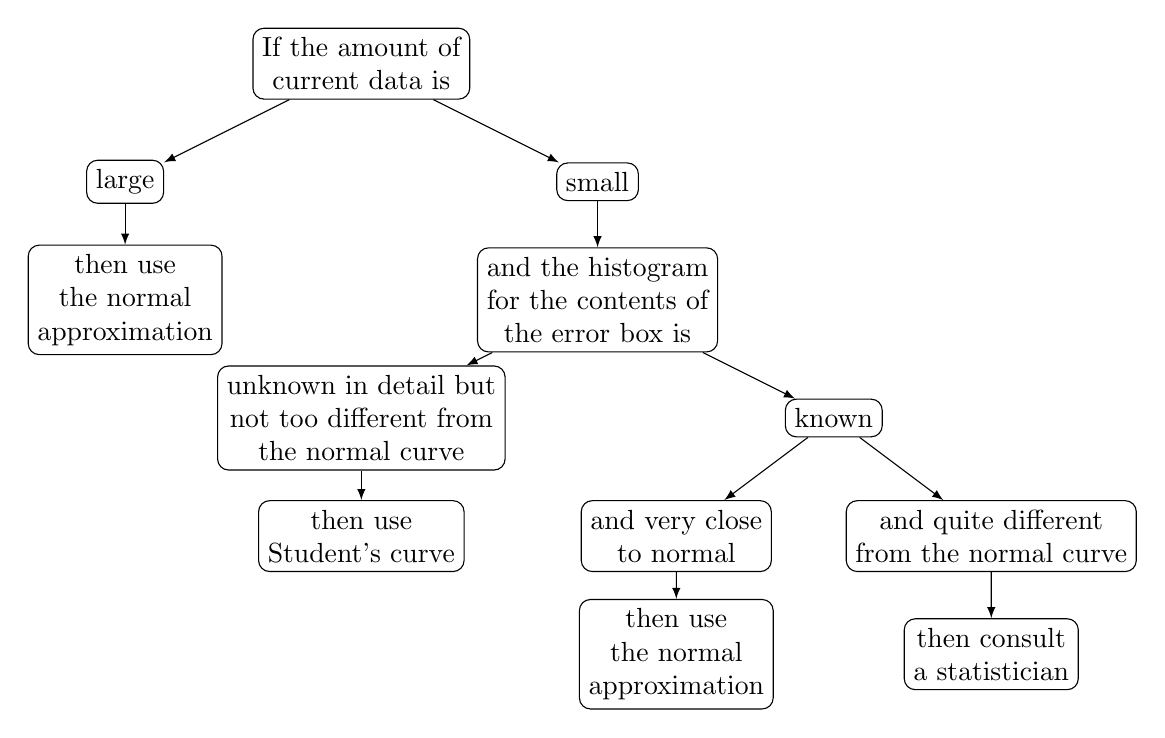
\begin{tikzpicture}[
    every node/.style={draw, align=center, rectangle, rounded corners}, % 'align=center' is required for line breaks to work
    edge from parent/.style={draw,-latex},
    level 1/.style={sibling distance=60mm},
    level 2/.style={sibling distance=60mm},
    level 3/.style={sibling distance=6cm},
    level 4/.style={sibling distance=4cm}
]
\node {If the amount of\\current data is}
    child {node {large}
        child {node {then use\\the normal\\approximation}}
    }
    child {node {small}
        child {node {and the histogram\\for the contents of\\the error box is}
            child {node {unknown in detail but\\not too different from\\the normal curve}
                child {node {then use\\Student's curve}}
            }
            child {node {known}
                child {node {and very close\\to normal}
                    child {node {then use\\the normal\\approximation}}
                }
                child {node {and quite different\\from the normal curve}
                    child {node {then consult\\a statistician}}
                }
            }
        }
    };
\end{tikzpicture}

\end{document}